\section{多元函数积分学}

\paragraph{\boxed{\text{积分转换}}}

\subsubsection{交换积分次序}

\paragraph{\boxed{\text{直角坐标系}}} \leavevmode \medskip

\textbf{例题:}交换积分次序$\int_0^1\textrm{d}x\int_0^{x^2}f(x,y)\,\textrm{d}y+\int_1^3\textrm{d}x\int_0^{\frac{1}{2}(3-x)}f(x,y)\,\textrm{d}y$。

解:已知积分区域分为两个部分。将$X$型变为$Y$型。画出图形可以知道$y\in(0,1)$,$x$的上下限由$y=x^2$和$y=\dfrac{1}{2}(3-x)$转化为$\sqrt{y}$和$3-2y$。

所以转换为$\int_0^1\textrm{d}y\int_{\sqrt{y}}^{3-2y}f(x,y)\,\textrm{d}x$。

\paragraph{\boxed{\text{极坐标系}}} \leavevmode \medskip

\textbf{例题:}对$\int_{-\frac{\pi}{4}}^{\frac{\pi}{2}}\textrm{d}\theta\int_0^{2\cos\theta}f(r\cos\theta,r\sin\theta)r\,\textrm{d}r$交换积分次序。

解:对于极坐标的积分次序交换需要利用直角坐标系来画图了解,特别是对于$r$的上下限。

对$\theta=\dfrac{\pi}{2}$变为$y$轴,$\theta=-\dfrac{\pi}{4}$变为$y=-x$。

对$r=2\cos\theta$变为$xy$的表达式,$r^2=2\cos\theta$,即$x^2+y^2=2x$,$(x-1)^2+y^2=1$。

所以所得到的$\sigma$为一个圆割去一个扇形。

\begin{minipage}{0.625\linewidth}
    
    交换积分次序后就需要以一个长度以极点为圆心做圆,切割$\sigma$。

    由$\sigma$可知取长度$\sqrt{2}$可以切分。

    所以$\sigma$可以分为左边的$\sigma_1$和右边的$\sigma_2$。
\end{minipage}
\hfill
\begin{minipage}{0.25\linewidth}
    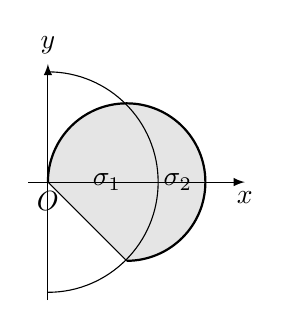
\begin{tikzpicture}[scale=1]
        \draw [black, thick, smooth, domain=0:1,fill=gray!20] (1,-1) arc (-90:180:1);
        \draw (0,0) -- (1,-1);
        \draw (0,-1.4) arc (-90:90:1.4);
        \draw[-latex](-0.25,0) -- (2.5,0) node[below]{$x$};
        \draw[-latex](0,-1.5) -- (0,1.5) node[above]{$y$};
        \filldraw[black] (0,0) node[below]{$O$};
        \filldraw (0.75,0) node{$\sigma_1$};
        \filldraw (1.65,0) node{$\sigma_2$};
    \end{tikzpicture}
\end{minipage}

$\sigma_1$的$r\in[0,\sqrt{2}]$,$\sigma_2$的$r\in[\sqrt{2},2]$。

$\sigma_1$的$\theta$下限是$y=-x$这条边,即$\theta=-\dfrac{\pi}{4}$,上限是$r=2\cos\theta$这个圆,则$\theta=\arccos\dfrac{r}{2}$。

$\sigma_2$的$\theta$界限都是是$r=2\cos\theta$这个圆,此时$r>0$恒成立,但是上限是上半部分$\theta>0$,而下限是下半部分$\theta<0$,即上限$\theta=\arccos\dfrac{r}{2}$,所以下限为$\theta=-\arccos\dfrac{r}{2}$。

综上交换积分次序结果为:

$\int_0^{\sqrt{2}}r\,\textrm{d}r\int_{-\frac{\pi}{4}}^{\arccos\frac{r}{2}}f(r\cos\theta,r\sin\theta)\textrm{d}\theta+\int_{\sqrt{2}}^2r\,\textrm{d}r\int_{-\arccos\frac{r}{2}}^{\arccos\frac{r}{2}}f(r\cos\theta,r\sin\theta)\textrm{d}\theta$。

\subsubsection{极直互化}

\textbf{例题:}将$I=\int_0^{\frac{\sqrt{2}}{2}R}e^{-y^2}\textrm{d}y\int_0^ye^{-x^2}\,\textrm{d}x+\int_{\frac{\sqrt{2}}{2}R}^Re^{-y^2}\,\textrm{d}y\int_0^{\sqrt{R^2-y^2}}e^{-x^2}\,\textrm{d}x$转换为极坐标系并计算结果。

解:首先根据积分上下限得到积分区域$D=\left\{0\leqslant y\leqslant\dfrac{\sqrt{2}}{2}R,0\leqslant x\leqslant y\right\}\cup\left\{\dfrac{\sqrt{2}}{2}R\leqslant y\leqslant R,0\leqslant x\leqslant\sqrt{R^2-y^2}\right\}$,$D$为一个八分之一圆的扇形。

根据$x=r\cos\theta$,$y=r\sin\theta$替换得到$D=\left\{(x,y)\bigg|0\leqslant r\leqslant R,\dfrac{\pi}{4}\leqslant\theta\leqslant\dfrac{\pi}{2}\right\}$。

又$e^{-y^2}\cdot e^{-x^2}=e^{-(x^2+y^2)}=e^{-r^2}$。

$\therefore I=\int_{\frac{\pi}{4}}^{\frac{\pi}{2}}\textrm{d}\theta\int_0^Re^{-r^2}r\,\textrm{d}r$。

\paragraph{\boxed{\text{二重积分计算}}}

二重积分若是累次积分形式出现,则计算可以使用上面两种方法简便运算。

\subsubsection{交换积分次序}

主要用于直角坐标系。

当按照当前的积分次序无法算出时需要更换积分次序。主要是看$f(x,y)$是对$x$先积分更简单还是对$y$先积分更简单。

\textbf{例题:}求$\int_0^1\textrm{d}y\int_{\arcsin y}^{\pi-\arcsin y}\cos^2x\,\textrm{d}x$。

解:首先直接对这个式子直接计算,$\cos^2x=\dfrac{1}{2}(1+\cos2x)$,原式$=\dfrac{1}{2}\int_0^1(\pi-2y-\arcsin y)\textrm{d}y$。根本无法解出。

考虑交换积分次序,首先求$\sigma$,$y\in[0,1]$,$x\in[\arcsin y,\pi-\arcsin y]$,则$\sin x=y$,$y=\sin(\pi-x)=\sin x$即$x\in[0,\sin x]$。

将积分区域换成$X$型:$x\in[0,\pi]$,$y\in[0,\sin x]$。

$\int_0^\pi\cos^2x\,\textrm{d}x\int_0^{\sin x}\textrm{d}y=\int_0^\pi\cos^2x\sin x\,\textrm{d}x=-\int_0^\pi\cos^2x\,\textrm{d}(\cos x)=-\dfrac{\cos^3x}{3}\bigg|_0^\pi\\=\dfrac{2}{3}$。

\subsubsection{积分性质}

直角坐标系和极坐标系都可以使用。

\paragraph{\boxed{\text{直角坐标系}}} \leavevmode \medskip

主要是一般对称性(积分区域关于$x$轴对称若$y$奇则为0,关于$y$轴对称若$x$奇则为0)和轮换对称性(积分区域关于$y=x$对称则$xy$可以互换)。

\paragraph{\boxed{\text{极坐标系} }}\leavevmode \medskip

主要就是指一般对称性(画图可知)。

\textbf{例题:}求曲线$r^2=2ax^2\cos2\theta$($a>0$)所围图形面积。

解:即求$\iint\limits_D\textrm{d}x\textrm{d}y$。重点就是求$D$,已知$r$的表达式,要求$\theta$的取值范围。

又$r^2>0$,$x^2>0$,$a>0$,所以$\cos2\theta\geqslant0$,$-\dfrac{\pi}{4}\leqslant\theta\leqslant\dfrac{\pi}{4}$,$\dfrac{3\pi}{4}\leqslant\theta\leqslant\dfrac{5\pi}{4}$。

由对称性,所以$=4\int_0^{\frac{\pi}{4}}\textrm{d}\theta\int_0^{a\sqrt{2\cos2\theta}}r\,\textrm{d}r=4a^2\int_0^{\frac{\pi}{4}}\cos2\theta\,\textrm{d}\theta=2a^2$。

\subsubsection{切分区域}

主要用于直角坐标系转为极坐标系。

将不规则的区域划分为圆域。

\textbf{例题:}设$D=\{(x,y)|0\leqslant x\leqslant1,0\leqslant y\leqslant1\}$,求$\displaystyle{\iint\limits_D\dfrac{\textrm{d}x\textrm{d}y}{\sqrt{x^2+y^2}}}$。

解:由$f(x,y)=\dfrac{1}{\sqrt{x^2+y^2}}$,知道可以使用极坐标系来表示,但是$D$是一个正方形,无法用圆来简单表示。

又$D$可以从$y=x$切割为两个部分,所以令下三角形为$D_1$,$\displaystyle{\iint\limits_D\dfrac{\textrm{d}x\textrm{d}y}{\sqrt{x^2+y^2}}}=2\displaystyle{\iint\limits_{D_1}\dfrac{\textrm{d}x\textrm{d}y}{\sqrt{x^2+y^2}}}$。

所以$0\leqslant y$和$y=x$可以确定$\theta\in\left[0,\dfrac{\pi}{4}\right]$,$0\leqslant x\leqslant1$可以确定$r$上界为$x=1$,即$r\cos\theta=1$,即$r=\dfrac{1}{\cos\theta}$,确定$r\in\left[0,\dfrac{1}{\cos\theta}\right]$。

所以$=2\int_0^{\frac{\pi}{4}}\textrm{d}\theta\int_0^{\frac{1}{\cos\theta}}\textrm{d}r=2\int_0^{\frac{\pi}{4}}\dfrac{\textrm{d}\theta}{\cos\theta}=2\ln(\sec\theta+\tan\theta)|_0^{\frac{\pi}{4}}=2\ln(1+\sqrt{2})$。

即对二重积分求导,需要将二重积分化为一重积分。

\subsubsection{坐标轴移动}

主要用于直角坐标系转为极坐标系。

面对$D$为一个圆的部分区域,而圆心不在原点,则可以坐标轴移动让圆心到原点上,从而方便积分,本质就是换元。

\textbf{例题:}设积分区域$D=\{(x,y)\vert x^2+y^2\leqslant2x+2y\}$,求$\iint_D(x^2+xy+y^2)\textrm{d}\sigma$。

解:$D$为$(x-1)^2+(y-1)^2\leqslant\sqrt{2}$,即圆心在$(1,1)$的圆,极坐标系无法表示,所以必须平移坐标轴。

令$x-1=u$,$y-1=v$,$x=u+1$,$y=v+1$,此时$D'=\{(u,v)|u^2+v^2\leqslant2\}$。

$\iint\limits_D(x^2+xy+y^2)\textrm{d}\sigma=\iint\limits_{D'}[(u+1)^2+(u+1)(v+1)+(v+1)^2]\textrm{d}u\textrm{d}v=\iint\limits_{D'}[u^2+uv+v^2+3(u+v)+3]\textrm{d}u\textrm{d}v=\iint\limits_{D'}(u^2+v^2)\textrm{d}u\textrm{d}v+\iint\limits_{D'}[uv+3(u+v)]\textrm{d}u\textrm{d}v+3\iint_{D'}\textrm{d}u\textrm{d}v$。

由于$uv+3(u+v)$是关于$u$或$v$的奇函数,且$D'$关于$uv$轴都对称,所以积分值为0。且根据二重积分的几何意义$\iint\limits_{D'}\textrm{d}u\textrm{d}v=S_{D'}=2\pi$。

所以$\iint_D(x^2+xy+y^2)\textrm{d}\sigma=\iint\limits_{D'}(u^2+v^2)\textrm{d}u\textrm{d}v+6\pi$。

转换为极坐标系,$u=r\cos\theta$,$v=r\sin\theta$,则$D'=\{(r,\theta)|0\leqslant\theta\leqslant2\pi,0\leqslant r\leqslant\sqrt{2}\}$。

$\iint\limits_{D'}(u^2+v^2)\textrm{d}u\textrm{d}v=\int_0^{2\pi}\textrm{d}\theta\int_0^{\sqrt{2}}r^3\,\textrm{d}r=2\pi\int_0^{\sqrt{2}}r^3\,\textrm{d}r=\dfrac{\pi}{2}(\sqrt{2})^4=2\pi$。

所以原式$=2\pi+6\pi=8\pi$。

若积分区域$\sigma$关于$x=k_1$或$y=k_2$对称,则当$f(x,y)$含有$x-k_1$或$y-k_2$因式时重积分值为0。

\textbf{例题:}设$D:x^2+y^2\leqslant2x+2y$,求$\iint\limits_Dxy\,\textrm{d}x\textrm{d}y$。

解:本题目使用直角坐标系和极坐标系都不好做。所以需要利用积分性质,对$D$进行平移等操作。

利用平移,由于$D:(x-1)^2+(y-1)^2=2$,令$x=1+r\cos\theta$,$y=1+r\sin\theta$,则利用极坐标,$r\in[0,\sqrt{2}]$,$\theta\in[0,2\pi]$,$=\int_0^{2\pi}\textrm{d}\theta\int_0^{\sqrt{2}}((1+r\cos\theta)(1+r\sin\theta)r)\textrm{d}r=\int_0^{2\pi}\textrm{d}\theta\int_0^{\sqrt{2}}(1+r\sin\theta+r\cos\theta+r^2\sin\theta\cos\theta)r\,\textrm{d}r$,又将$\sin\theta$和$\cos\theta$对$\theta$在$[0,2\pi]$进行积分全部为0,所以直接把后面的全消掉,变为$\int_0^{2\pi}\textrm{d}\theta\int_0^{\sqrt{2}}r\,\textrm{d}r=2\pi$。

\subsubsection{极限化为二重积分}

类似极限转换为定积分,有$\lim\limits_{n\to\infty}\dfrac{1}{n^2}\sum\limits_{i=1}^n\sum\limits_{j=1}f\left(\dfrac{i}{n},\dfrac{j}{n}\right)=\int_0^1\textrm{d}x\int_0^1f(x,y)\,\textrm{d}y$:

\begin{enumerate}
    \item 先提出$\dfrac{1}{n^2}$。
    \item 凑出$\dfrac{i}{n}$和$\dfrac{j}{n}$。
    \item 写出$\int_0^1\textrm{d}x$、$\int_0^1f(x,y)\,\textrm{d}y$,其中$\dfrac{1}{n^2}$没有了,将所有$\dfrac{i}{n}$换为$x$,$\dfrac{j}{n}$换为$y$。
\end{enumerate}

\textbf{例题:}求$I=\lim\limits_{n\to\infty}\sum\limits_{i=1}^n\sum\limits_{j=1}^n\dfrac{1}{\left(1+\dfrac{i}{n}\right)(n^2+j^2)}$。

解:首先提出$\dfrac{1}{n^2}$,正好在分母右边等式中$=\lim\limits_{n\to\infty}\sum\limits_{i=1}^n\sum\limits_{j=1}^n\dfrac{1}{\left(1+\dfrac{i}{n}\right)(1+\dfrac{j^2}{n^2})}\dfrac{1}{n^2}$。

已完全化为$\dfrac{i}{n}$和$\dfrac{j}{n}$,所以$=\displaystyle{\int_0^1\dfrac{1}{1+x}\textrm{d}x\int_0^1\dfrac{1}{1+y^2}\textrm{d}y}$。

$=\ln(1+x)\vert_0^1\arctan y\vert_0^1=\dfrac{\pi}{4}\ln2$。

\subsubsection{二重积分极限}

即对存在二重积分的式子求极限。当对二重积分求极限时基本上都需要使用洛必达法则对积分求导。

令中间的定积分为$g(x)$,并记住$(\int_{f(x)}^{g(x)}h(t)\,\textrm{d}t)'=(g'(x)-f'(x))h(x)$。上下限最好换为$x$和$0$。

\textbf{例题:}求$\lim\limits_{t\to0^+}\dfrac{1}{t^6}\int_0^t\textrm{d}x\int_x^t\sin(xy)^2\textrm{d}y$。

解:这个式子求极限必然使用洛必达法则,而$\int_0^t\textrm{d}x\int_x^t\sin(xy)^2\textrm{d}y$里面那层定积分的上下限不规整,所以更换积分次序变成$\int_0^t\textrm{d}y\int_0^x\sin(xy)^2\textrm{d}x$。

对其求导$\int_0^t[\int_0^x\sin(xy)^2\textrm{d}x]\textrm{d}y$,由于该层积分变量为$y$,令$\int_0^x\sin(xy)^2\textrm{d}x=g(y)$,所以$=\int_0^tg(y)\,\textrm{d}y$,对其求导得$g(t)$,里面的$y$全部用$t$替换$=\int_0^x\sin(xt)^2\textrm{d}x$。

$=\lim\limits_{t\to0^+}\dfrac{\int_0^t\textrm{d}x\int_x^t\sin(xy)^2\textrm{d}y}{t^6}=\lim\limits_{t\to0^+}\dfrac{\int_0^t\sin(xt)^2\textrm{d}x}{6t^5}=\lim\limits_{t\to0^+}\dfrac{\int_0^t\sin(xt)^2\textrm{d}(xt)}{6t^6}$。

由于$x$和$t$都是变量,所以令$xt=u$,$x=\dfrac{u}{t}$,$u\in(0,t^2)$,$=\lim\limits_{t\to0^+}\dfrac{\int_0^{t^2}\sin u^2\textrm{d}u}{6t^6}=\lim\limits_{t\to0^+}\dfrac{2t\sin t^4}{36t^5}=\lim\limits_{t\to0^+}\dfrac{t^5}{18t^5}=\dfrac{1}{18}$。

\subsubsection{广义极坐标系}

广义极坐标系是对极坐标系的延伸,极坐标系是广义坐标系的特例。极坐标系是基于直线和圆周进行积分,而广义极坐标系可以对圆锥曲线进行积分。

当对面积为非圆形进行积分时可以使用广义极坐标系。

$\iint\limits_{D_1}f(x,y)\,\textrm{d}x\textrm{d}y$,$x=g(u,v)$,$y=h(u,v)$,换元为$\iint\limits_{D_2}f(g(u,v),h(u,v))\vert J\vert\,\textrm{d}u\textrm{d}v$,$J$为雅可比行列式,可以看作代表$(x,y)$坐标系的面积微元和$(u,v)$坐标系的面积微元的比率:

$J=\left[\begin{array}{cc}
    \dfrac{\partial x}{\partial u} & \dfrac{\partial x}{\partial v} \\
    \dfrac{\partial y}{\partial u} & \dfrac{\partial y}{\partial v}
\end{array}\right]$。

\textbf{例题:}设$D:\dfrac{x^2}{a}+\dfrac{y^2}{b}\leqslant1$,求$\iint\limits_Dy^2\,\textrm{d}x\textrm{d}y$。

解:令$x=ar\cos\theta$,$y=br\sin\theta$,所以$D'$为$0\leqslant r\leqslant 1$,$0\leqslant\theta\leqslant2\pi$。

变换雅可比行列式$J=\dfrac{\partial(x,y)}{\partial(r,\theta)}=\left\vert\begin{array}{cc}
    \dfrac{\partial x}{\partial r} & \dfrac{\partial x}{\partial\theta} \\
    \dfrac{\partial y}{\partial r} & \dfrac{\partial y}{\partial\theta}
\end{array}\right\vert=\left\vert\begin{array}{cc}
    a\cos\theta & -ar\sin\theta \\
    b\sin\theta & br\cos\theta
\end{array}\right\vert=abr$。

所以$I=\iint\limits_{D'}(br\sin\theta)^2\vert J\vert\,\textrm{d}r\textrm{d}\theta=\int_0^{2\pi}\textrm{d}\theta\int_0^1b^2r^2\sin^2\theta\cdot abr\,\textrm{d}r=\dfrac{\pi ab^3}{4}$。

\paragraph{\boxed{\text{二重积分等式}}}

\subsubsection{函数}

\textbf{例题:}设$f(x,y)$为连续函数,且$f(x,y)=\dfrac{1}{\pi}\sqrt{x^2+y^2}\iint\limits_{x^2+y^2\leqslant1}f(x,y)\,\textrm{d}\sigma+y^2$,求$f(x,y)$。

解:$\because f(x,y)$为连续函数,所以其在区间上可积且是一个常数。

令$\iint\limits_{x^2+y^2\leqslant1}f(x,y)\,\textrm{d}\sigma=A$。对$f(x,y)=\dfrac{A}{\pi}\sqrt{x^2+y^2}+y^2$两边积分:

$A=\dfrac{A}{\pi}\iint\limits_{x^2+y^2\leqslant1}\sqrt{x^2+y^2}\,\textrm{d}\sigma+\iint\limits_{x^2+y^2\leqslant1}y^2\,\textrm{d}\sigma$,令$x=r\cos\theta$,$y=r\sin\theta$:

$A=\dfrac{A}{\pi}\int_0^{2\pi}\textrm{d}\theta\int_0^1r^2\,\textrm{d}r+\int_0^{2\pi}\sin^2\theta\textrm{d}\theta\int_0^1r^3\,\textrm{d}r=\dfrac{2A}{3}+\dfrac{\pi}{4}$。$A=\dfrac{3}{4}\pi$。

则代入原式$f(x,y)=\dfrac{3}{4}\sqrt{x^2+y^2}+y^2$。

\subsubsection{极限}

\textbf{例题:}设$g(x)$有连续的导数,且$g(0)=0$,$g'(0)=a\neq0$,$f(x,y)$在$(0,0)$的某邻域内连续,求$\lim\limits_{r\to0^+}\dfrac{\iint\limits_{x^2+y^2\leqslant r^2}f(x,y)\,\textrm{d}x\textrm{d}y}{g(r^2)}$。

解:已知对于这个积分式子中$f(x)$和$g(x)$都是未定式,不可能求出具体的值,所以不能再用二重积分直接计算。

面对这种未定式我们希望把这个式子变成我们已知的式子,也应该与$r$相关。此时我们可以想到二重积分中值定理。

根据二重积分中值定理$\iint\limits_{x^2+y^2\leqslant r^2}f(x,y)\,\textrm{d}x\textrm{d}y=\pi r^2f(\xi,\eta)$,其中$(\xi,\eta)$为圆域$x^2+y^2\leqslant r^2$上的点,所以$\lim\limits_{r\to0^+}f(\xi,\eta)=f(0,0)$。

$=\lim\limits_{r\to0^+}\dfrac{\pi r^2f(\xi,\eta)}{g(r^2)}=\lim\limits_{r\to0^+}\dfrac{\pi f(0,0)2r}{2rg'(r^2)}=\lim\limits_{r\to0^+}\dfrac{\pi f(0,0)}{g'(r^2)}=\dfrac{\pi f(0,0)}{g'(0)}=\dfrac{\pi f(0,0)}{a}$。

\subsubsection{求导}

\paragraph{\boxed{\text{二重积分不等式}}}

即对二重积分进行对比。

\subsubsection{同积分域}

同一积分域上二重积分大小的比较,只要比较在该区间被积函数值的大小。

\subsubsection{同积分函数}

同一积分函数上二重积分大小的比较,要比较函数域的大小,也要注意在函数域上被积函数的符号。

\textbf{例题:}设积分区域$D_1=\{(x,y)|x^2+y^2\leqslant1\}$、$D_2=\{(x,y)|x^2+y^2\leqslant2\}$、$D_3=\left\{(x,y)|\dfrac{1}{2}x^2+y^2\leqslant1\right\}$、$D_4=\left\{(x,y)|x^2+\dfrac{1}{2}y^2\leqslant1\right\}$。\\记$I_i=\iint\limits_{D_i}\left[1-\left(x^2+\dfrac{1}{2}y^2\right)\right]\textrm{d}\sigma$($i=1,2,3,4$),求$\max\{I_1,I_2,I_3,I_4\}$。

解:已知$D_1$、$D_2$分别为半径1和$\sqrt{2}$的圆,而$D_3$、$D_4$分别为横着和竖着的椭圆。可以画出图像。

被积函数$f(x,y)=1-\left(x^2+\dfrac{1}{2}y^2\right)$为连续函数,只有在$D_4$上才能保证完全为正,以外的地方为负值。

所以$D_1\subset D_4$,所以$I_1<D_4$。对于$D_2$更大,$D_4\subset D_2$,但是多余的左右部分是负值,积分值会在$D_4$的基础上减去这部分的值,同理$D_3$和$D_4$一个是横的椭圆一个是竖的椭圆,其积分值只有中间交叉的部分,还要减去两边多余的部分。

所以$I_4$最大。

\paragraph{\boxed{\text{一重积分化二重积分}}}

对于一重积分的计算或证明可能比较有难度,如两个关于$x$的函数的一重积分乘积计算,可以将其中一个$x$当作$y$,从而将一重积分的乘积变为二重积分。

\subsubsection{乘积化不等式}

\textbf{例题:}$f(x)$为恒大于0的连续函数,证明$\displaystyle{\int_a^bf(x)\,\textrm{d}x\cdot\int_a^b\dfrac{1}{f(x)}\textrm{d}x\geqslant(b-a)^2}$。

解:首先观察这个式子,右边是积分上下限的差的乘积,左边是两个积分的乘积,看上去貌似没什么关系,而且积分式子给出的是一个未定式$f(x)$,所以不能直接求左边值再比较大小,他们之间一定存在着某种关系。

式子左边的两个函数互为倒数,所以应该要尝试将这两个式子乘在一起来利用基本不等式计算,即将一重积分乘积变为二重积分。

对于一重积分而言只是一个自变量,对于二重积分而言就变成了两个自变量,需要令其中一个$f(x)$变为$y$,所以$xy$的积分区域都是一样的$[a,b]$,所以设$D=\{(x,y)\vert a\leqslant x\leqslant b,a\leqslant y\leqslant b\}$。

$I=\displaystyle{\int_a^bf(x)\,\textrm{d}x\cdot\int_a^b\dfrac{1}{f(x)}\textrm{d}x}=\int_a^bf(x)\,\textrm{d}x\cdot\int_a^b\dfrac{1}{f(y)}\textrm{d}y=\iint\limits_D\dfrac{f(x)}{f(y)}\textrm{d}x\textrm{d}y$。

$I=\displaystyle{\int_a^bf(x)\,\textrm{d}x\cdot\int_a^b\dfrac{1}{f(x)}\textrm{d}x}=\int_a^bf(y)\,\textrm{d}y\cdot\int_a^b\dfrac{1}{f(x)}\textrm{d}x=\iint\limits_D\dfrac{f(y)}{f(x)}\textrm{d}x\textrm{d}y$。

$\therefore I=\displaystyle{\dfrac{1}{2}\left[\iint\limits_D\left[\dfrac{f(x)}{f(y)}+\dfrac{f(y)}{f(x)}\right]\textrm{d}x\textrm{d}y\right]\geqslant\dfrac{1}{2}\iint\limits_D2\sqrt{\dfrac{f(x)}{f(y)}\cdot\dfrac{f(y)}{f(x)}}\textrm{d}x\textrm{d}y=}\\\displaystyle{\dfrac{1}{2}\iint\limits_D2\textrm{d}x\textrm{d}y}=(b-a)^2$。

\subsubsection{乘积简化计算}

\textbf{例题:}求$\int_0^{+\infty}e^{-x^2}\,\textrm{d}x$。

解:对于这个一重积分首先看到$e^{x^2}$,肯定会想到将其幂次降低。使用分部积分法对$e^{e^2}$求导这个幂次不会降低,使用换元法$x=\sqrt{t}$会得到$\dfrac{1}{\sqrt{t}}$从而无法处理,所以这些都不能计算,那么该怎么办?

看到$x^2$就能想到$x^2+y^2$的形式,这样就是一个极坐标系的二重积分,所以尝试将一重积分变成二重积分,即再乘一个以$y$为自变量的原式。

设$I=\int_0^{+\infty}e^{-x^2}\,\textrm{d}x$,显然$I>0$,将$x$换成$y$:

$I^2=\int_0^{+\infty}e^{-x^2}\,\textrm{d}x\cdot\int_0^{+\infty}e^{-x^2}\,\textrm{d}x=\int_0^{+\infty}e^{-x^2}\,\textrm{d}x\cdot\int_0^{+\infty}e^{-y^2}\,\textrm{d}y$

$=\displaystyle{\iint\limits_{\substack{0\leqslant x\leqslant+\infty\\0\leqslant y\leqslant+\infty}}e^{-(x^2+y^2)}\,\textrm{d}x\textrm{d}y}$,令$x=r\cos\theta$,$y=r\sin\theta$:

$=\displaystyle{\int_0^\frac{\pi}{2}\textrm{d}\theta\int_0^{+\infty}e^{-r^2}r\,\textrm{d}r=\dfrac{\pi}{2}\left(-\dfrac{1}{2}\right)\int_0^{+\infty}e^{-r^2}\,\textrm{d}(-r^2)=-\dfrac{\pi}{4}e^{-r^2}\bigg\vert_0^{+\infty}}=\dfrac{\pi}{4}$。

$\therefore I=\dfrac{\sqrt{\pi}}{2}$。

\paragraph{二重积分应用}

\subsubsection{体积}

\subsubsection{形心公式}

直角坐标系和极坐标系的形心公式都是一样的,使用极坐标系可以转换。

\textbf{例题:}求曲线$ay=x^2$与$x+y=2a$所围平面区域$D$的形心坐标。

解:根据表达式可知有两个交点$(-2a,4a)$、$(a,a)$,形心公式:

$\overline{x}=\dfrac{\iint\limits_Dx\,\textrm{d}\sigma}{\iint\limits_D\textrm{d}\sigma}=\dfrac{\int_{-2a}^ax\,\textrm{d}x\int_{\frac{x^2}{a}}^{-x+2a}\textrm{d}y}{\int_{-2a}^a\,\textrm{d}x\int_{\frac{x^2}{a}}^{-x+2a}\textrm{d}y}=\dfrac{\int_{-2a}^a(-\dfrac{x^3}{a}-x^2+2ax)\textrm{d}x}{\int_{-2a}^a(-\dfrac{x^2}{a}-x+2a)\textrm{d}x}=-\dfrac{1}{2}a$

$\overline{y}=\dfrac{\iint\limits_Dy\,\textrm{d}\sigma}{\iint\limits_D\textrm{d}\sigma}=\dfrac{\int_{-2a}^a\,\textrm{d}x\int_{\frac{x^2}{a}}^{-x+2a}y\textrm{d}y}{\int_{-2a}^a\,\textrm{d}x\int_{\frac{x^2}{a}}^{-x+2a}\textrm{d}y}=\dfrac{\dfrac{1}{2}\int_{-2a}^a(-\dfrac{x^4}{4}+x^2-4ax+4a^2)}{\int_{-2a}^a(-\dfrac{x^2}{a}-x+2a)\textrm{d}x}=\dfrac{8}{5}a$

\subsection{弧长曲线积分}

\subsection{坐标曲线积分}

\paragraph{定积分法}

\paragraph{\boxed{\text{二重积分法}}}

\subsubsection{补全区域}

即$L$不能构成一个完整的域,就需要按照路径对区域进行补全,然后减去这个曲线积分值。

\subsubsection{不可导点}

即$D$中存在不可导的点,需要以不可导点为圆心做圆对$D$进行切割。

\textbf{例题:}$I=\displaystyle{\oint\limits_L\dfrac{x\textrm{d}y-y\textrm{d}}{x^2+y^2}}$,$L$为不过原点的闭曲线。

解:$P=-\dfrac{y}{x^2+y^2}$,$Q=\dfrac{x}{x^2+y^2}$。$\dfrac{\partial Q}{\partial x}=\dfrac{y^2-x^2}{(x^2+y^2)^2}$,$\dfrac{\partial P}{\partial y}=\dfrac{y^2-x^2}{(x^2+y^2)^2}$,从而$\dfrac{\partial Q}{\partial x}\equiv\dfrac{\partial P}{\partial y}$。但是此时$(x,y)\neq(0,0)$,所以格林公式无法使用。

若$(0,0)\notin D$,则可以使用格林公式,$I=\iint\limits_D0\,\textrm{d}\sigma=0$。

若$(0,0)\in D$,不可以使用格林公式,所以重新对$D$进行划分,令$L_0:x^2+y^2=r^2$,其中$r>0$且$L_0$不超过$D$,$L_0$为逆时针。中间的环为$D_1$,最里侧的圆为$D_2$。

所以对中间的环$D_1$使用格林公式:$\oint_{L+L_0^-}=\iint_{D_1}\left(\dfrac{\partial Q}{\partial x}-\dfrac{\partial P}{\partial y}\right)\textrm{d}\sigma=0$。

$\therefore\oint\limits_L+\oint\limits_{L_0^-}=\oint\limits_L-\oint\limits_{L_0}=0$,$\oint_L=\oint_{L_0}$。

$I=\displaystyle{\oint\limits_{L_0}\dfrac{x\textrm{d}y-y\textrm{d}x}{x^2+y^2}=\dfrac{1}{r^2}\oint\limits_{L_0}x\,\textrm{d}y-y\,\textrm{d}x=\dfrac{2}{r^2}\iint\limits_{D_2}\textrm{d}\sigma=2\pi}$。

\textbf{例题:}计算曲线积分$\oint\limits_L\dfrac{x\textrm{d}y-y\textrm{d}x}{4^x2+y^2}$,其中$L$是以点$(1,0)$为圆心,$R\geqslant1$为半径的圆,取逆时针方向。

解:由于是逆时针在$L$上,所以是正向:$=\displaystyle{\oint\limits_{L^+}\left(\dfrac{-y}{4x^2+y^2}\textrm{d}x+\dfrac{x}{4x^2+y^2}\textrm{d}y\right)}$。

又对于$L$所围成的圆面$D$,因为$4x^2+y^2\neq0$,所以$(0,0)$应该被挖去。

因为逆时针的方向下挖去这个点做的运动顺时针是负方向的,所以令其为$C^-$。

又因为格林公式$\oint\limits_{L^++C^-}P\,\textrm{d}x+Q\,\textrm{d}y=\displaystyle{\iint\limits_D\left(\dfrac{\partial Q}{\partial x}-\dfrac{\partial P}{\partial y}\right)\textrm{d}\sigma}=$\\$\displaystyle{\iint\limits_D\left(\dfrac{4x^2+y^2-3x^2}{(4x^2+y^2)^2}-\dfrac{-(4x^2+y^2)+2y^2}{(4x^2+y^2)^2}\right)\textrm{d}\sigma}=0$。旋度为0。

$=\oint\limits_{L^++C^-}-\oint\limits_{C^-}=0-\oint\limits_{C^-}=\oint\limits_{C^+}$。取$C:4x^2+y^2=\delta^2$,$\delta$为一个足够小的常数。(分母取$\delta^2$)

$=\displaystyle{\oint\limits_{C^+}\left(\dfrac{-y}{4x^2+y^2}\textrm{d}x+\dfrac{x}{4x^2+y^2}\textrm{d}y\right)}=\displaystyle{\oint\limits_{C^+}\left(\dfrac{-y}{\delta^2}\textrm{d}x+\dfrac{x}{\delta^2}\textrm{d}y\right)}$

$=\dfrac{1}{\delta^2}\oint\limits_{C^+}-y\,\textrm{d}x+x\,\textrm{d}y$,利用格林公式,$C^+$所成区域为$D'$:$\dfrac{1}{\delta^2}\oint\limits_{D'}(1-(-1))\,\textrm{d}\sigma=\dfrac{2}{\delta^2}D'=\dfrac{2}{\delta^2}\pi\dfrac{\delta}{2}\delta=\pi$。
